%-%-%-%-%-%-%-%-%-%-%-%-%-%-%-%-%-%-%-%-%-%-%-%-%-%-%-%-%-%-%-%-%-%-%-%-%-%-%
%%% MAIN DOCUMENT %%%

%-%-%-%-%-%-%-%-%-%-%-%-%-%-%-%-%-%-%-%-%-%-%-%-%-%-%-%-%-%-%-%-%-%-%-%-%-%-%

\documentclass[12pt, oneside]{book}
\usepackage{xcolor}
\usepackage{minted}

% \usepackage[T1]{fontenc}

\usepackage{draculatheme}
\newcommand{\documentTheme}{draculafg}
\newcommand{\documentLogo}{images/ML_logo_v2.png}
\newcommand{\documentBigLogo}{images/ML_logo_v2.png}
% \usemintedstyle{dracula}

% \newcommand{\documentBigLogo}{images/Hendrix Logo.png}
% \newcommand{\documentLogo}{images/small logo.png}
% \newcommand{\documentTheme}{black}

%%% AESTHETICS %%%
%-%-%-%-%-%-%-%-%-%-%-%-%-%-%-%-%-%-%-%-%-%-%-%-%-%-%-%-%-%-%-%-%-%-%-%-%-%-%


%%% Dimensions and Spacing %%%
\usepackage[margin=1in]{geometry}
% \setlength{\parindent}{0pt}
\usepackage{setspace}
\usepackage{mathtools}
\linespread{1}
\usepackage{listings}
\usepackage{tikz}
\usetikzlibrary{shapes,backgrounds,calc,patterns,positioning}
\usepgflibrary{shadings}
\usepackage{pgfkeys}
\usepackage{pdftexcmds}
\usepackage{shellesc}
\usepackage{algorithm, algorithmic, xspace}
%%% Define new colors %%%
% \definecolor{draculapink}{rgb}{0.96, 0.51, 0.16}

% Normal colors
\definecolor{xred}{HTML}{BD4242}
\definecolor{xblue}{HTML}{4268BD}
\definecolor{xgreen}{HTML}{52B256}
\definecolor{xpurple}{HTML}{7F52B2}
\definecolor{xorange}{HTML}{FD9337}
\definecolor{xdotted}{HTML}{999999}
\definecolor{xgray}{HTML}{777777}
\definecolor{xcyan}{HTML}{80F5DC}
\definecolor{xpink}{HTML}{F690EA}
\definecolor{xgrayblue}{HTML}{49B095}
\definecolor{xgraycyan}{HTML}{5AA1B9}

% Dark colors
\colorlet{xdarkred}{red!85!black}
\colorlet{xdarkblue}{xblue!85!black}
\colorlet{xdarkgreen}{xgreen!85!black}
\colorlet{xdarkpurple}{xpurple!85!black}
\colorlet{xdarkorange}{xorange!85!black}
\definecolor{xdarkcyan}{HTML}{008B8B}
\colorlet{xdarkgray}{xgray!85!black}

% Very dark colors
\colorlet{xverydarkblue}{xblue!50!black}

% Document-specific colors
\colorlet{normaltextcolor}{black}
\colorlet{figtextcolor}{xblue}

% Enumerated colors
\colorlet{xcol0}{black}
\colorlet{xcol1}{xred}
\colorlet{xcol2}{xblue}
\colorlet{xcol3}{xgreen}
\colorlet{xcol4}{xpurple}
\colorlet{xcol5}{xorange}
\colorlet{xcol6}{xcyan}
\colorlet{xcol7}{xpink!75!black}

% Blue-Purple (should just used colorbrewer...)
\definecolor{xrainbow0}{HTML}{e41a1c}
\definecolor{xrainbow1}{HTML}{a24057}
\definecolor{xrainbow2}{HTML}{606692}
\definecolor{xrainbow3}{HTML}{3a85a8}
\definecolor{xrainbow4}{HTML}{42977e}
\definecolor{xrainbow5}{HTML}{4aaa54}
\definecolor{xrainbow6}{HTML}{629363}
\definecolor{xrainbow7}{HTML}{7e6e85}
\definecolor{xrainbow8}{HTML}{9c509b}
\definecolor{xrainbow9}{HTML}{c4625d}
\definecolor{xrainbow10}{HTML}{eb751f}
\definecolor{xrainbow11}{HTML}{ff9709}

%------- %
% XHFILL %
%------- %



%%% Chapter Headings %%%

\newcommand{\gradientrule}{
    \begin{tikzpicture}
        \shade[left color=draculapink, right color=black, middle color=gray] (0,0) rectangle (\linewidth,0.4pt);
    \end{tikzpicture}
}

\usepackage[Glenn]{fncychap}
\ChTitleVar{\bfseries\scshape\color{\documentTheme}} % Needed for Dracula theme
\ChNumVar{\large\selectfont\color{\documentTheme}} % Needed for Dracula theme
\ChNameVar{\large\color{\documentTheme}} % Needed for Dracula theme
\usepackage{xpatch}

% \xpatchcmd{\DOCH}
%   {\mghrulefill}{\gradientrule\mghrulefill}
%   {}{\PatchFailed}
% \xpatchcmd{\DOTI}
%   {\mghrulefill}{\gradientrule\mghrulefill}
%   {}{\PatchFailed}
% \xpatchcmd{\DOTIS}
%   {\mghrulefill}{\gradientrule\mghrulefill}
%   {}{\PatchFailed}

\xpatchcmd\DOCH
{\mghrulefill}{\color{draculapink}\mghrulefill}
{}{\PatchFailed}
\xpatchcmd\DOTI
{\mghrulefill}{\color{draculapink}\mghrulefill}
{}{\PatchFailed}
\xpatchcmd\DOTIS
{\mghrulefill}{\color{draculapink}\mghrulefill}
{}{\PatchFailed}


% \usepackage[Bjornstrup]{fncychap}

% \newcommand{\gradient}[1]{
% \begin{tikzpicture}
%     \node (rect) at (0,0) [fill=blue,,path fading=East,minimum width=\linewidth,minimum height=2.5cm] {};
%     \node(title)[above left = 10pt and 10pt of rect.south east, anchor=south east, font=\CTV] {\textcolor{horange}{#1}};
%     \ifnum \thechapter>0\node[left = 10pt of rect.north east,  anchor=center, font=\CNoV] {\textcolor{horange}{\thechapter}};\fi%
% \end{tikzpicture}%
% \vskip 40pt
% }


% \renewcommand{\DOCH}{}
% \renewcommand{\DOTI}[1]{\gradient{#1}}
% \renewcommand{\DOTIS}[1]{\gradient{#1}}

%% Change Chapter Heading Placement %%
\usepackage{etoolbox}
\makeatletter
\patchcmd{\@makechapterhead}{\vspace*{50\p@}}{\vspace*{-20\p@}}{}{}
\patchcmd{\@makeschapterhead}{\vspace*{50\p@}}{\vspace*{-20\p@}}{}{}
\patchcmd{\DOTI}{\vskip 80\p@}{\vskip 40\p@}{}{}
\patchcmd{\DOTIS}{\vskip 40\p@}{\vskip 0\p@}{}{}
\makeatother

\usepackage{titlesec}

% \usepackage[explicit]{titlesec}
% \newcommand*\chapterlabel{}\pmod
% \titleformat{\chapter}
%   {\gdef\chapterlabel{}
%    \normalfont\sffamily\Huge\bfseries\scshape}
%   {\gdef\chapterlabel{\thechapter\ }}{0pt}
%   {\begin{tikzpicture}[remember picture,overlay]
%     \node[yshift=-3cm] at (current page.north west)
%       {\begin{tikzpicture}[remember picture, overlay]
%         \draw[fill=LightSkyBlue] (0,0) rectangle
%           (\paperwidth,3cm);
%         \node[anchor=east,xshift=.9\paperwidth,rectangle,
%               sharp corners=downhill=20pt,inner sep=11pt,
%               fill=MidnightBlue]
%               {\color{white}\chapterlabel#1};
%        \end{tikzpicture}
%       };
%    \end{tikzpicture}
%   }
% \titlespacing*{\chapter}{0pt}{50pt}{-60pt}

% \usepackage[Conny]{fncychap}
% \usepackage[Rejne]{fncychap}
% \ChNameVar{\bfseries}  % Makes the chapter "Chapter #" bold
% \ChNumVar{\bfseries}   % Makes the chapter number bold
% \ChTitleVar{\bfseries} % Makes the chapter title bold
% % Define a custom color, for example:
% \definecolor{mycolor}{RGB}{0,128,255}

% % Redefine the chapter style in Rejne to change the line colors
% \makeatletter
% \ChRuleWidth{2pt}   % Change the thickness of the lines
% \renewcommand{\DOCH}{%
%   \vspace*{-50\p@}% Moves the chapter title up/down if needed
%   {\color{mycolor} \hrule \@chapapp{} \space \thechapter \hrule}% Customizes the chapter header with color
% }
% \renewcommand{\DOTI}[1]{%
%   \vskip 20\p@ % Adjusts the space above the title
%   \bfseries #1\par % Embolden the title
%   \vskip 20\p@ % Adjusts the space below the title
% }
% \makeatother

% %% Change Chapter Heading Placement %%
% \usepackage{etoolbox}
% \makeatletter
% \patchcmd{\@makechapterhead}{\vspace*{50\p@}}{\vspace*{-20\p@}}{}{}
% \patchcmd{\@makeschapterhead}{\vspace*{50\p@}}{\vspace*{-20\p@}}{}{}
% \patchcmd{\DOTI}{\vskip 80\p@}{\vskip 40\p@}{}{}
% \patchcmd{\DOTIS}{\vskip 40\p@}{\vskip 0\p@}{}{}
% \makeatother

\renewcommand{\thesection}{\thechapter.\arabic{section}} %% Chapter.Section Numbering

% Section title: 90% opacity
\titleformat{\section}
  {\normalfont\Large\bfseries\color{draculapink!100}}
  {\thesection}{1em}{}

% Subsection title: 80% opacity
\titleformat{\subsection}
  {\normalfont\large\bfseries\color{draculapink!75}}
  {\thesubsection}{1em}{}

% Subsubsection title: 70% opacity
\titleformat{\subsubsection}
  {\normalfont\normalsize\bfseries\color{draculapink!50}}
  {\thesubsubsection}{1em}{}

%%% FIGURES %%%
\usepackage{graphicx}  
% \numberwithin{figure}{section}
\usepackage{float}
\usepackage{caption}

%%% Hyperlinks %%%
\usepackage{hyperref}
% \definecolor{draculacyan}{HTML}{f58026}
\hypersetup{
	colorlinks=true,
	linkcolor=draculacyan,
	filecolor=draculacyan,      
	urlcolor=draculacyan,
}


%% Headers and Footers %%
\usepackage{fancyhdr} % This should be set AFTER setting up the page geometry
\pagestyle{fancy} % options: empty , plain , fancy
\renewcommand{\chaptermark}[1]{\markboth{\thechapter.\ #1}{}}
\fancyhead[R]{\leftmark}
\fancyhead[L]{Paul Beggs}
% \fancyhead[C]{\includegraphics[height=1cm]{\documentLogo}} % Use for Dracula
\usepackage{xpatch}
\xpretocmd\headrule{\color{draculapink}}{}{\PatchFailed}
\setlength{\footskip}{0.5in}
\setlength{\headheight}{18.5764pt}


%%%%% Colored Boxes %%%%%
\usepackage{tcolorbox}
\tcbuselibrary{skins}
\tcbuselibrary{theorems}
% \tcbuselibrary{minted}
\newcounter{BoxCounter}
\usepackage{dingbat}

%-%-%-%-%-%-%-%-%-%-%-%-%-%-%-%-%-%-%-%-%-%-%-%-%-%-%-%-%-%-%-%-%-%-%-%-%-%-%

%% MATH PACKAGES, ENVIRONMENTS, COMMANDS %%
%-%-%-%-%-%-%-%-%-%-%-%-%-%-%-%-%-%-%-%-%-%-%-%-%-%-%-%-%-%-%-%-%-%-%-%-%-%-%
%You'll need your own packages, theorem types, and commands.

\usepackage{fix-cm}
\usepackage{amsmath,amsthm} 
\usepackage{mathtools}
\usepackage{amssymb}
\usepackage[framemethod=tikz]{mdframed}
\usepackage{mathrsfs}
\usepackage{changepage}
\usepackage{footmisc}
\usepackage{multicol}
\usepackage{slashed}
\usepackage{enumerate}
\usepackage{braket}
\usepackage{booktabs}
\usepackage{enumitem}
\usepackage{kantlipsum}  %This package lets us generate random text for example purposes.
\usepackage{pgfplots}


%%% Custom Commands %%%
% Natural Numbers 
\newcommand{\N}{\mathbb{N}}

% Whole Numbers
\newcommand{\W}{\mathbb{W}}

% Integers
\newcommand{\Z}{\mathbb{Z}}

% Rational Numbers
\newcommand{\Q}{\mathbb{Q}}

% Real Numbers
\newcommand{\R}{\mathbb{R}}

% Complex Numbers
\newcommand{\C}{\mathbb{C}}

\newcommand{\I}{\mathbb{I}}

\newcommand{\pfs}{\noindent\makebox[\linewidth]{\rule{\textwidth}{0.4pt}}\vspace{0.5cm}}

\newcommand{\mysqrt}[1]{%
  \mathpalette\foo{#1}%
}
\newcommand{\dmysqrt}[1]{%
  \mathpalette\foodisplay{#1}%
}

% !TeX spellcheck = off
\newcommand{\foo}[2]{%
  % #1: math style, #2: content
  \sbox0{$#1\sqrt{#2}$}% Measure the size of the standard sqrt in the current style
  \begin{tikzpicture}[baseline=(sqrt.base)]
    \node[inner sep=0, outer sep=0] (sqrt) {$#1\sqrt{#2}$}; % Use the current math style
    \draw([yshift=-0.045em]sqrt.north east) -- ++(0,-0.5ex); % Draw the tick
  \end{tikzpicture}%
}
% !TeX spellcheck = off
\newcommand{\foodisplay}[2]{%
  % #1: math style, #2: content
  \sbox0{$#1\sqrt{#2}$}% Measure the size of the standard sqrt in the current style
  \begin{tikzpicture}[baseline=(sqrt.base)]
    \node[inner sep=0, outer sep=0] (sqrt) {$\displaystyle\sqrt{#2}$}; % Force displaystyle
    \draw[line width=0.4pt] ([yshift=-0.044em]sqrt.north east) -- ++(0,-0.5ex); % Draw the tick
  \end{tikzpicture}%
}


% \newcommand{}{\marginnote{
\includegraphics[width=2em]{caution.png}}}

\newmdenv[
  topline=false,
  bottomline=true,
  rightline=false,
  leftline=true,
  linewidth=1.5pt,
  linecolor=black, % default color, will be overridden in custom commands
  backgroundcolor=draculabg, % Needed for Dracula theme
  fontcolor=\documentTheme, % Needed for Dracula theme
  innertopmargin=0pt,
  innerbottommargin=5pt,
  innerrightmargin=10pt,
  innerleftmargin=10pt,
  leftmargin=0pt,
  rightmargin=0pt,
  skipabove=\topsep,
  skipbelow=\topsep,
]{customframedproof}

\newenvironment{proofpart}[2][black]{
    \begin{mdframed}[
        topline=false,
        bottomline=false,
        rightline=false,
        leftline=true,
        linewidth=1pt,
        linecolor=#1!40, % Custom color
        % innertopmargin=10pt,
        % innerbottommargin=10pt,
        innerleftmargin=10pt,
        innerrightmargin=10pt,
        leftmargin=0pt,
        rightmargin=0pt,
        % skipabove=\topsep,
        % skipbelow=\topsep%
    ]
    \noindent
    \begin{minipage}[t]{0.08\textwidth}%
        \textbf{#2}%
    \end{minipage}%
    \begin{minipage}[t]{0.90\textwidth}%
        \begin{adjustwidth}{0pt}{0pt}%
}{
    \end{adjustwidth}
    \end{minipage}
    \end{mdframed}
}

% Define a new environment 'proofscratch' for Proof and Scratch Paper
\newenvironment{proofscratch}[2]{%
    \begin{mdframed}[
        topline=false,
        bottomline=false,
        rightline=false,
        leftline=false,
        backgroundcolor=draculabg, % Background color for Dracula theme
        fontcolor=\documentTheme,       % Font color for Dracula theme
        innerleftmargin=-6pt,
        innertopmargin=0pt,
        leftmargin=0pt,
        rightmargin=0pt,
        skipabove=\topsep,
        skipbelow=\topsep,
    ]
    % % Begin TikZ picture for the vertical dotted line
    % \begin{tikzpicture}[overlay, remember picture]
    %     % Draw a vertical dotted line at approximately the center of the mdframed width
    %     \draw[dotted, thick] ([xshift=0.005\linewidth]current bounding box.north west) -- ([xshift=0.005\linewidth]current bounding box.south west);
    % \end{tikzpicture}%
    % % Create the left minipage for Proof
    \begin{minipage}[t]{0.47\textwidth}%
        \noindent\textit{Proof.} #1 \hfill \(\qed\)
    \end{minipage}%
    \hfill
    % Create the right minipage for Scratch Paper
    \begin{minipage}[t]{0.47\textwidth}%
        \textit{Scratch Paper.} #2
    \end{minipage}%
}{
    \end{mdframed}
}

\newcommand{\nobulletitem}[1]{\item {\itshape #1}}

\newlist{nobullet}{itemize}{10}
\setlist[nobullet,1]{label=}
\setlist[nobullet,2]{label=}
\setlist[nobullet,3]{label=}
\setlist[nobullet,4]{label=}

\newenvironment{tipbox}
  {%
    \par\noindent%
    % Top dashed line (using \textwidth)
    \tikz[baseline]{\draw[dash pattern=on 3pt off 2pt, line width=0.5pt, color=draculapurple] (0,0) -- (\textwidth,0);}%
    \par\vspace{0.65em}%
    \noindent\textbf{\textcolor{draculapurple}{TIP:}}\quad%
  }
  {%
    \par%
    % Bottom dashed line
    \noindent%
    \tikz[baseline]{\draw[dash pattern=on 3pt off 2pt, line width=0.5pt, color=draculapurple] (0,0) -- (\textwidth,0);}%
    \par\vspace{0.35em}
  }

\newenvironment{notebox}
  {%
    \par\noindent%
    % Top dashed line (using \textwidth)
    \tikz[baseline]{\draw[dash pattern=on 3pt off 2pt, line width=0.5pt, color=draculagreen] (0,0) -- (\textwidth,0);}%
    \par\vspace{0.65em}%
    \noindent\textbf{\textcolor{draculagreen}{NOTE:}}\quad%
  }
  {%
    \par%
    % Bottom dashed line
    \noindent%
    \tikz[baseline]{\draw[dash pattern=on 3pt off 2pt, line width=0.5pt, color=draculagreen] (0,0) -- (\textwidth,0);}%
    \par\vspace{0.35em}
  }

\newenvironment{warningbox}
  {%
    \par\noindent%
    % Top dashed line (using \textwidth)
    \tikz[baseline]{\draw[dash pattern=on 3pt off 2pt, line width=0.5pt, color=draculared] (0,0) -- (\textwidth,0);}%
    \par\vspace{0.65em}%
    \noindent\textbf{\textcolor{draculared}{WARNING:}}\quad%
  }
  {%
    \par%
    % Bottom dashed line
    \noindent%
    \tikz[baseline]{\draw[dash pattern=on 3pt off 2pt, line width=0.5pt, color=draculared] (0,0) -- (\textwidth,0);}%
    \par\vspace{0.35em}
  }



\newcommand{\sol}[1]{
    \begin{customframedproof}[linecolor=draculapink!75,]
        \begin{solution}
        #1
        \end{solution}
    \end{customframedproof}
}

\def \proofDistance {10pt}
\newenvironment{solution}
  {\textit{Solution.}}

\newcommand{\disabs}[1]{\ensuremath{\left|#1\right|}}
\newcommand{\limn}{\lim_{n \rightarrow \infty}}
\newcommand{\limx}[2]{\lim_{x \rightarrow #1}#2}

\newcommand{\limc}[1]{\lim_{x \rightarrow c}#1}

\newcommand{\ninn}{n \in \N}

\newcommand{\mb}[1]{\mathbf{#1}}

\newcommand{\limsupn}[1]{\limsup_{n\rightarrow \infty}#1}
\newcommand{\liminfn}[1]{\liminf_{n\rightarrow \infty}#1}

\renewcommand{\theenumi}{\alph{enumi}} 
\renewcommand{\labelenumi}{(\theenumi)}

\newcommand{\proj}{\text{proj}}

\newcommand{\p}{\partial}

\newcommand{\dydx}{\frac{dy}{dx}}
\newcommand{\dxdy}{\frac{dx}{dy}}
\newcommand{\dydt}{\frac{dy}{dt}}
\newcommand{\dxdt}{\frac{dx}{dt}}
\newcommand{\dzdt}{\frac{dz}{dt}}

\newcommand{\barNotationT}[1]{\bigg|_{t = #1}}

\newcommand{\cyanit}[1]{\textit{\textcolor{cyan}{#1}}}

\newcommand{\brackett}[1]{\left\langle #1 \right\rangle}

\newcommand{\norm}[1]{\left\lVert \mathbf{#1}\right\rVert}

\newcommand{\imb}{\mb{i}}
\newcommand{\jmb}{\mb{j}}
\newcommand{\kmb}{\mb{k}}
\newcommand{\rmb}{\mb{r}}
\newcommand{\umb}{\mb{u}}

\newcommand{\vecfuc}[2]{\mb{#1}(#2)}
\newcommand{\dvecfuc}[2]{\mb{#1}'(#2)}
\newcommand{\normdvecfuc}[2]{\|\mb{#1}'(#2)\|}

\newcommand{\quoteAuthor}[1]{\hspace*{9cm} \textemdash #1}

\newcommand{\variablename}[1]{\textcolor{draculacyan}{\texttt{#1}}}


% end of preamble
%-%-%-%-%-%-%-%-%-%-%-%-%-%-%-%-%-%-%-%-%-%-%-%-%-%-%-%-%-%-%-%-%-%-%-%-%-%-%

\begin{document}

\numberwithin{BoxCounter}{section}


%-%-%-%-%-%-%-%-%-%-%-%-%-%-%-%-%-%-%-%-%-%-%-%-%-%-%-%-%-%-%-%-%-%-%-%-%-%-%
%%% COVER PAGE %%%
%-%-%-%-%-%-%-%-%-%-%-%-%-%-%-%-%-%-%-%-%-%-%-%-%-%-%-%-%-%-%-%-%-%-%-%-%-%-%

% Do not use all caps.
\newcommand{\titlestandin}{Machine Learning Notes (Book 2)}
\newcommand{\cussubtitle}{``An Introduction To Statistical Learning''}
% Date format should be like: "January 1, 2001"

%-%-%-%-%-%-%-%-%-%-%-%-%-%-%-%-%-%-%-%-%-%-%-%-%-%-%-%-%



\begin{titlepage}
    \begin{center}

        \vspace*{-2cm}
        \begin{figure}[h!]
            \centering
            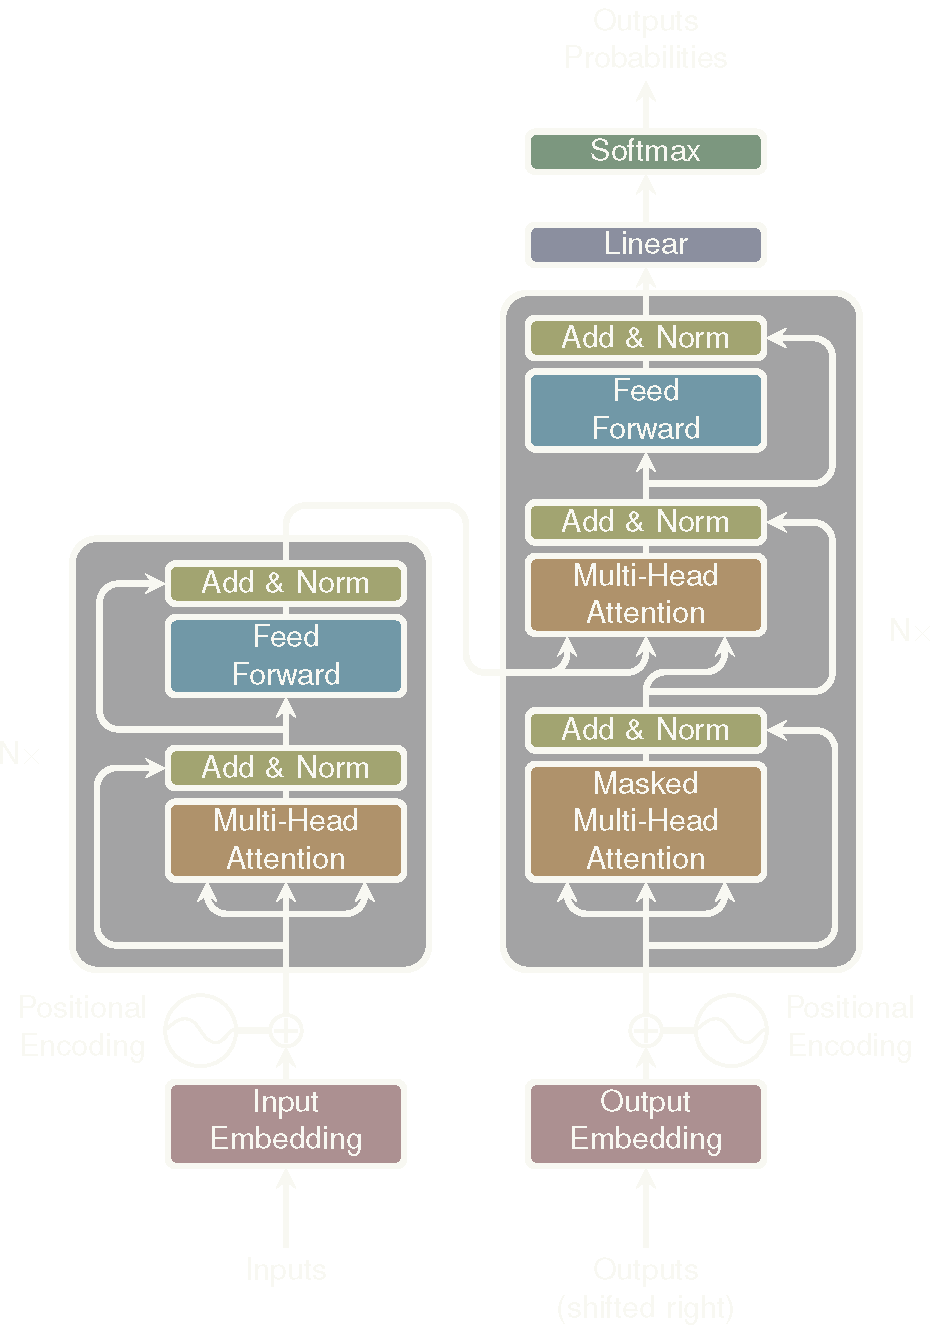
\includegraphics[width=0.6\textwidth]{images/ML_logo_v3.png}\\
            \caption{``The Transformer'' Recreated in TikZ from \href{https://proceedings.neurips.cc/paper_files/paper/2017/file/3f5ee243547dee91fbd053c1c4a845aa-Paper.pdf}{``Attention Is All You Need''}}
        \end{figure}

        % Horizontal line above the title in 'horange' color
        \textcolor{draculapink}{\rule{\textwidth}{1.0pt}}

        \vspace{2em}

        {\huge \textbf{\titlestandin}}

        \vspace{1em} % Space between the title and the bottom line

        \textcolor{draculapink}{\rule{\textwidth}{1.0pt}}

        \vspace*{1\baselineskip}

        {\LARGE \textbf{\cussubtitle}}

        \begin{large}
            \vspace*{2\baselineskip}

            \emph{Author} \\[1ex]
            %Submitted by \\[\baselineskip]
            {\Large Paul Beggs \\ \par} % Editor list
            {\href{mailto:PaulBeggs03@gmail.com}{{PaulBeggs03@gmail.com}}}\\ % Editor affiliation

        \end{large}
    \end{center}
\end{titlepage}
\pagebreak

%-%-%-%-%-%-%-%-%-%-%-%-%-%-%-%-%-%-%-%-%-%-%-%-%-%-%-%-%-%-%-%-%-%-%-%-%-%-%

%%% Table of Contents %%%


% -%-%-%-%-%-%-%-%-%-%-%-%-%-%-%-%-%-%-%-%-%-%-%-%-%-%-%-%-%-%-%-%-%-%-%-%-%-%

% Helper command to fix header for double paged ToC.
% Temporarily adjust section marks for Table of Contents
\begin{spacing}{1} % Can change spacing between entries in TOC
    \renewcommand{\contentsname}{\Large\textbf{Table of Contents}} % Can rename here
    \markboth{}{} % Clear the header marks for TOC
    \pagestyle{fancy} % Ensure fancy style is active
    \fancyhead[R]{Table of Contents} % Set TOC-specific header manually
    \tableofcontents
    \addtocontents{toc}{\protect\enlargethispage{\baselineskip}}
\end{spacing}

% Reset the headers to default for the rest of the document
\fancyhead[R]{\leftmark}




% -%-%-%-%-%-%-%-%-%-%-%-%-%-%-%-%-%-%-%-%-%-%-%-%-%-%-%-%-%-%-%-%-%-%-%-%-%-%

\chapter{Introduction}
\vspace*{-0.25in}
\section{Notation and Simple Matrix Algebra}
\label{sec:notation}

The following text is taken directly from the book:

Choosing notation for a textbook is always a difficult task. For the most part, we adopt the same notational conventions as ESL. 

We will use \( n \) to represent the number of distinct data points, or observations, in our sample. We will let \( p \) denote the number of variables that are available for use in making predictions. 

For example, the \variablename{wage} data set consists of 11 variables for 3,000 people, so we have \( n = 3000 \) observations and \( p = 11 \) variables (such as \variablename{year}, \variablename{age}, \variablename{race}, and more). 

Note that throughout this book, we indicate variable names using colored font: \variablename{Variable Name}.

In some examples, \( p \) might be quite large, such as on the order of thousands or even millions; this situation arises quite often, for example, in the analysis of modern biological data or web-based advertising data.

\subsection{Notation}

In general, we let \( x_{ij} \) represent the value of the \( j \)th variable for the \( i \)th observation, where \( i = 1, 2, \ldots, n \) and \( j = 1, 2, \ldots, p \). 

Throughout this book, \( i \) will be used to index the samples or observations (from 1 to \( n \)) and \( j \) will be used to index the variables (from 1 to \( p \)).

We let \( \mathbf{X} \) denote an \( n \times p \) matrix whose \( (i,j) \)th element is \( x_{ij} \). That is,
\[
\mathbf{X} = 
\begin{pmatrix}
x_{11} & x_{12} & \cdots & x_{1p} \\
x_{21} & x_{22} & \cdots & x_{2p} \\
\vdots & \vdots & \ddots & \vdots \\
x_{n1} & x_{n2} & \cdots & x_{np}
\end{pmatrix}.
\]

For readers who are unfamiliar with matrices, it is useful to visualize \( \mathbf{X} \) as a spreadsheet of numbers with \( n \) rows and \( p \) columns.

\subsection{Row and Column Vectors}

At times we will be interested in the rows of \( \mathbf{X} \), which we write as \( \mathbf{x}_1, \mathbf{x}_2, \ldots, \mathbf{x}_n \). Here \( \mathbf{x}_i \) is a vector of length \( p \), containing the \( p \) variable measurements for the \( i \)th observation. That is,
\begin{equation}
\mathbf{x}_i = 
\begin{pmatrix}
x_{i1} \\
x_{i2} \\
\vdots \\
x_{ip}
\end{pmatrix}.
\end{equation}

For example, for the \variablename{wage} data, \( \mathbf{x}_i \) is a vector of length 11, consisting of year, age, race, and other values for the \( i \)th individual.

At other times we will instead be interested in the columns of \( \mathbf{X} \), which we write as \( \mathbf{x}_{1}, \mathbf{x}_{2}, \ldots, \mathbf{x}_{p} \). Each is a vector of length \( n \). That is,
\[
\mathbf{x}^{(j)} =
\begin{pmatrix}
x_{1j} \\
x_{2j} \\
\vdots \\
x_{nj}
\end{pmatrix}.
\]

For example, for the \variablename{wage} data, \( \mathbf{x}_{1} \) contains the \( n = 3000 \) values for year.

Using this notation, the matrix \( \mathbf{X} \) can also be written as
\[
\mathbf{X} = 
\begin{pmatrix}
\mathbf{x}_{1} & \mathbf{x}_{2} & \cdots & \mathbf{x}_{p}
\end{pmatrix},
\quad \text{or} \quad
\mathbf{X} = 
\begin{pmatrix}
\mathbf{x}_1^T \\
\mathbf{x}_2^T \\
\vdots \\
\mathbf{x}_n^T
\end{pmatrix}.
\]

Here, the superscript \( ^{T} \) denotes the transpose of a matrix or vector. So, for example, 
\[
\mathbf{X}^T = 
\begin{pmatrix}
x_{11} & x_{21} & \cdots & x_{n1} \\
x_{12} & x_{22} & \cdots & x_{n2} \\
\vdots & \vdots & \ddots & \vdots \\
x_{1p} & x_{2p} & \cdots & x_{np}
\end{pmatrix},
\quad
\mathbf{x}_i^T = 
\begin{pmatrix}
x_{i1} & x_{i2} & \cdots & x_{ip}
\end{pmatrix}.
\]

\subsection{Output Variable}

We use \( y_i \) to denote the \( i \)th observation of the variable on which we wish to make predictions, such as \variablename{wage}. Hence, we write the set of all \( n \) observations in vector form as
\[
\mathbf{y} = 
\begin{pmatrix}
y_1 \\
y_2 \\
\vdots \\
y_n
\end{pmatrix}.
\]

Then our observed data consists of the pairs 
\[
\{ (\mathbf{x}_1, y_1), (\mathbf{x}_2, y_2), \ldots, (\mathbf{x}_n, y_n) \},
\]
where each \( \mathbf{x}_i \) is a vector of length \( p \). (If \( p = 1 \), then \( \mathbf{x}_i \) is simply a scalar.)

\subsection{Vector and Matrix Notation}

\begin{itemize}
    \item A vector of length \( n \) is always denoted in lower-case bold font, e.g., \( \mathbf{a} = [a_1, a_2, \ldots, a_n]^T \).
    \item Vectors not of length \( n \) (such as feature vectors of length \( p \)) are denoted in lower-case normal font, e.g., \( a \).
    \item Scalars are denoted in lower-case normal font, e.g., \( a \).
    \item Matrices are denoted using bold capitals, such as \( \mathbf{A} \).
    \item Random variables are denoted using capital normal font, e.g., \( A \), regardless of their dimensions.
\end{itemize}

In rare cases where the use of lower-case normal font leads to ambiguity, we will clarify the intended use.

\subsection{Dimensions and Spaces}

To indicate the dimension of a particular object:

\begin{itemize}
    \item Scalar: \( a \in \mathbb{R} \)
    \item Vector of length \( k \): \( a \in \mathbb{R}^k \)
    \item Vector of length \( n \): \( a \in \mathbb{R}^n \)
    \item Matrix of size \( r \times s \): \( \mathbf{A} \in \mathbb{R}^{r \times s} \)
\end{itemize}

\subsection{Matrix Multiplication}

We have avoided using matrix algebra whenever possible. However, in a few instances it becomes too cumbersome to avoid it entirely. In these rare instances, it is important to understand the concept of multiplying two matrices. Suppose that \( \mathbf{A} \in \mathbb{R}^{r \times d} \) and \( \mathbf{B} \in \mathbb{R}^{d \times s} \). Then the product \( \mathbf{A}\mathbf{B} \) is an \( r \times s \) matrix, where the \( (i,j) \)th element is computed as
\[
(\mathbf{A}\mathbf{B})_{ij} = \sum_{k=1}^{d} a_{ik} b_{kj}.
\]

As an example, consider
\[
\mathbf{A} = 
\begin{pmatrix}
1 & 2 \\
3 & 4
\end{pmatrix}, \quad
\mathbf{B} = 
\begin{pmatrix}
5 & 6 \\
7 & 8
\end{pmatrix}.
\]

Then,
\begin{align*}
\mathbf{A}\mathbf{B} &= 
\begin{pmatrix}
1 \cdot 5 + 2 \cdot 7 & 1 \cdot 6 + 2 \cdot 8 \\
3 \cdot 5 + 4 \cdot 7 & 3 \cdot 6 + 4 \cdot 8
\end{pmatrix} \\
&=
\begin{pmatrix}
19 & 22 \\
43 & 50
\end{pmatrix}.
\end{align*}

Note that this operation produces an \( r \times s \) matrix. It is only possible to compute the product \( \mathbf{A}\mathbf{B} \) if the number of columns in \( \mathbf{A} \) (which is \( d \)) is equal to the number of rows in \( \mathbf{B} \) (which is also \( d \)).

\section{Organization of the Book}
\label{sec:organization}

Chapter 2 introduces the basic terminology and concepts behind statistical learning. This chapter also presents the K-nearest neighbor classifier, a very simple method that works surprisingly well on many problems. Chapters 3 and 4 cover classical linear methods for regression and classification. In particular, Chapter 3 reviews linear regression, the fundamental starting point for all regression methods. In Chapter 4 we discuss two of the most important classical classification methods, logistic regression and linear discriminant analysis.

A central problem in all statistical learning situations involves choosing the best method for a given application. Hence, in Chapter 5 we introduce cross-validation and the bootstrap, which can be used to estimate the accuracy of a number of different methods in order to choose the best one.

Much of the recent research in statistical learning has concentrated on non-linear methods. However, linear methods often have advantages over their non-linear competitors in terms of interpretability and sometimes also accuracy. Hence, in Chapter 6 we consider a host of linear methods, both classical and more modern, which offer potential improvements over standard linear regression. These include stepwise selection, ridge regression, principal components regression, and the lasso.

The remaining chapters move into the world of non-linear statistical learning. We first introduce in Chapter 7 a number of non-linear methods that work well for problems with a single input variable. We then show how these methods can be used to fit non-linear additive models for which there is more than one input. In Chapter 8, we investigate tree-based methods, including bagging, boosting, and random forests. Support vector machines, a set of approaches for performing both linear and non-linear classification, are discussed in Chapter 9. We cover deep learning, an approach for non-linear regression and classification that has received a lot of attention in recent years, in Chapter 10. Chapter 11 explores survival analysis, a regression approach that is specialized to the setting in which the output variable is censored, i.e. not fully observed.

In Chapter 12, we consider the unsupervised setting in which we have input variables but no output variable. In particular, we present principal components analysis, K-means clustering, and hierarchical clustering. Finally, in Chapter 13 we cover the very important topic of multiple hypothesis testing.

At the end of each chapter, we present one or more Python lab sections in which we systematically work through applications of the various methods discussed in that chapter. These labs demonstrate the strengths and weaknesses of the various approaches, and also provide a useful reference for the syntax required to implement the various methods. The reader may choose to work through the labs at their own pace, or the labs may be the focus of group sessions as part of a classroom environment. Within each Python lab, we present the results that we obtained when we performed the lab at the time of writing this book. However, new versions of Python are continuously released, and over time, the packages called in the labs will be updated. Therefore, in the future, it is possible that the results shown in the lab sections may no longer correspond precisely to the results obtained by the reader who performs the labs. As necessary, we will post updates to the labs on the book website.

\begin{table}[htbp]
    \centering
    \begin{tabular}{ll}
        \toprule
        \textbf{Name} & \textbf{Description} \\
        \midrule
        \variablename{Auto} & Gas mileage, horsepower, and other information for cars. \\
        \variablename{Bikeshare} & Hourly usage of a bike sharing program in Washington, DC. \\
        \variablename{Boston} & Housing values and other information about Boston census tracts. \\
        \variablename{BrainCancer} & Survival times for patients diagnosed with brain cancer. \\
        \variablename{Caravan} & Information about individuals offered caravan insurance. \\
        \variablename{Carseats} & Information about car seat sales in 400 stores. \\
        \variablename{College} & Demographic characteristics, tuition, and more for USA colleges. \\
        \variablename{Credit} & Information about credit card debt for 400 customers. \\
        \variablename{Default} & Customer default records for a credit card company. \\
        \variablename{Fund} & Returns of 2,000 hedge fund managers over 50 months. \\
        \variablename{Hitters} & Records and salaries for baseball players. \\
        \variablename{Khan} & Gene expression measurements for four cancer types. \\
        \variablename{NCI60} & Gene expression measurements for 64 cancer cell lines. \\
        \variablename{NYSE} & Returns, volatility, and volume for the New York Stock Exchange. \\
        \variablename{OJ} & Sales information for Citrus Hill and Minute Maid orange juice. \\
        \variablename{Portfolio} & Past values of financial assets, for use in portfolio allocation. \\
        \variablename{Publication} & Time to publication for 244 clinical trials. \\
        \variablename{Smarket} & Daily percentage returns for S\&P 500 over a 5-year period. \\
        \variablename{USArrests} & Crime statistics per 100,000 residents in 50 states of USA. \\
        \variablename{Wage} & Income survey data for men in central Atlantic region of USA. \\
        \variablename{Weekly} & 1,089 weekly stock market returns for 21 years. \\

        \bottomrule
    \end{tabular}
    \caption{A list of data sets needed to perform the labs and exercises in this textbook. All data sets are available in the \variablename{ISLR} package, with the exception of \variablename{USArrests}, which is part of the \variablename{R} distribution, but accessible from \variablename{Python}.}\label{tab:data_sets}
\end{table}

\setcounter{chapter}{1}





%-%-%-%-%-%-%-%-%-%-%-%-%-%-%-%-%-%-%-%-%-%-%-%-%-%-%-%-%-%-%-%-%-%-%-%-%-%-%
\end{document}
%-%-%-%-%-%-%-%-%-%-%-%-%-%-%-%-%-%-%-%-%-%-%-%-%-%-%-%-%-%-%-%-%-%-%-%-%-%-%

%-%-%-%-%-%-%-%-%-%-%-%-%-%-%-%-%-%-%-%-%-%-%-%-%-%-%-%-%-%-%-%-%-%-%-%-%-%-%